\documentclass{article}

\usepackage{amsmath}
\usepackage{mathtools}
\usepackage{amstext}
\usepackage{array}
\usepackage[long]{optidef}
\usepackage[backend=biber,
            url=false]{biblatex}
\usepackage{float}
\usepackage{tikz}
\usepackage{txfonts}
\usepackage[colorinlistoftodos]{todonotes}
\usepackage[long]{optidef}

  \addbibresource{ch1-2.bib}

  \usetikzlibrary{calc,matrix,decorations.markings,decorations.pathreplacing}
  \usetikzlibrary{positioning}

  \definecolor{colone}{gray}{0.7}
  \definecolor{coltwo}{gray}{0.6}
  \definecolor{colthree}{gray}{0.5}
  \definecolor{colfour}{gray}{0.9}
  \definecolor{colfive}{gray}{0.9}
  \definecolor{colsix}{gray}{0.9}
  \definecolor{colseven}{gray}{0.9}

  \tikzset{
  table/.style={
  matrix of nodes,
  row sep=-\pgflinewidth,
  column sep=-\pgflinewidth,
  nodes={rectangle,text width=2cm,align=center},
  text depth=1.25ex,
  text height=2.5ex,
  nodes in empty cells}
  }

  \tikzstyle{startstop} = [rectangle, minimum width=2cm, minimum height=1.5cm,text centered, draw=black]
  \tikzstyle{process} = [rectangle, minimum width=3cm, minimum height=1.5cm, text centered, draw=black]
  \tikzstyle{blank} = [circle, minimum width=0.1cm, minimum height=0.1cm, text centered, draw=white]
  \tikzstyle{arrow} = [thick,->,>=stealth]

\begin{document}

  \title{Chapter 2}

  \author{M. Repetto}

  \date{}

\maketitle

\begin{abstract}
  In the following paper is proposed a multi-objective model for goods allocation in a Green Supply Chain framework. The model builds on the concept of the open loop supply chain as suggested by Santoso with the integration of the Porter model for value chain, accounting for the costs of production using the Activity Based Cost accounting method (ABC). Finally, the model is enhanced to embrace the flow of recycled goods and therefore be a closed loop supply. Above every block of the recycling process, a series of environmental constraints have been included, that the firm has to comply, with respect to specific country regulation, or in case of a particular Corporate Environmental Responsibility policy. The resulting Weighted Fuzzy Goal Programming model is then solved and calibrated to the Decision Maker needs through Analytical Hierarchy Process.
\end{abstract}

\section{Introduction}
  Global Supply Chain Management (GSCM) is probably one of the most used terms when the discussion of how the firms are running their business is brought to the table nowadays. GSCM may be defined as the allocation of goods and services along a series of transnational companies' global network to maximize profits and minimize waste. As the Supply Chain Professionals puts it, the goal of GSCM is threefold and focuses on delivering: (a)the right product; (b)to the right place; (c)at the right time.
   Inside this very wide paradigm, the concept of logistics serves as the backbone; recalling that logistics is developed to be in charge of the movement of goods, service, and last but not least information from the sourcing of raw material, till it reaches the end customer.
  Along with these two concepts a third one sticks with them, the Green Supply Chain (GSC). This idea brought to light by a more advanced concern about environmental matters of the developed countries, forced the firms to be accountable for their negative externalities related to the environment in which they operate \cite{srivastava_green_2007}.

  However such legislation lacks from a point of view of legal constraints, setting only a few qualitative restrictions, poorly measurable by the enterprises or in some cases letting the customers pay for their environmental behavior toward waste disposition. These facts are inevitably leaving some degrees of freedom to the firms, on the other hand, is also important to notice that these are only seeds of legislation that show us how the long-term trend will be about the tolerance given to the behavior of firms with environmental concerns, a trend that in the future may require firms to set particular frameworks to be accountable for their environmental impact. Nowadays such effort is not achieved by the legal frameworks provided by the domestic legislators but by the Corporate Environmental Responsibility (CER), meaning that are the stakeholders to impose the companies to be more responsible on their day to day operations.

Speaking about the literature, is observable an emerging branch which deals with the Green Supply Chain Management, a new paradigm of Supply Chain Management whose aim is to keep under control the behavior of the firm during its operations, by applying policies such as Green Manufacturing and Re-manufacturing, Green Design etc... Because of that a Weighted Fuzzy Goal Programming model is proposed. In order to address such problems, following what proposed by literature, an enhanced model is proposed. such model, fixing quantitative and qualitative constraints to the recycled products handled by the company and tries to implement Decision Maker preferences  with respect to the recycling programs enacted by the firm apropos the WEEE directive. In the case under proposed, the choice was to opt for a networking electronic appliance business (i.e. hub, switch or router).  In order to measure such impact, the framework provided by the Activity Based Costing is used; such approach has the peculiarity to assess the marginal impact of any additional unit processed by the transnational firms, leaving outside the assessment any sunk cost.
\\
\\
The paper is organized into four parts, where two of them are devoted to a review of the existing literature and the last two, which are respectively model and result oriented. In the first of the literature sections a full overview of the Green Supply Chain framework will be given; at the same time the focus will be directed to the legal implications that are affecting both producer and distributors operating in the European Union. After this overview a deep analysis will be given on the state-of-the-art techniques used to model both Supply Chain Management and Logistics topics, focusing the attention on peculiar applications such as Stochastic Programming and Fuzzy Goal Programming. Ultimately the two sections devoted to the model will be used to state the model proposed with its objectives and constraints; then the model's weights will be subjected to sensitivity analysis with different scenarios and ultimately calibrated to the DM needs via AHP.

\pagebreak

\section{Green Supply Chain}
Green Supply Chain saw a steady growth of interest in many enterprises\cite{Diabat2011} as well as by academics; a growth that, looking to the data\cite{Strobel18}, reached its hype between the 2012 and 2014 (Figure \ref{fig:occurrence}) and that may be strengthen in the next years because of the increasing environmental concern. The main research fields interested by this phenomena are the ones involving environmental sciences, management, operational research and more generally green sustainable sciences\cite{Shan2018}  
\begin{figure}[ht]
	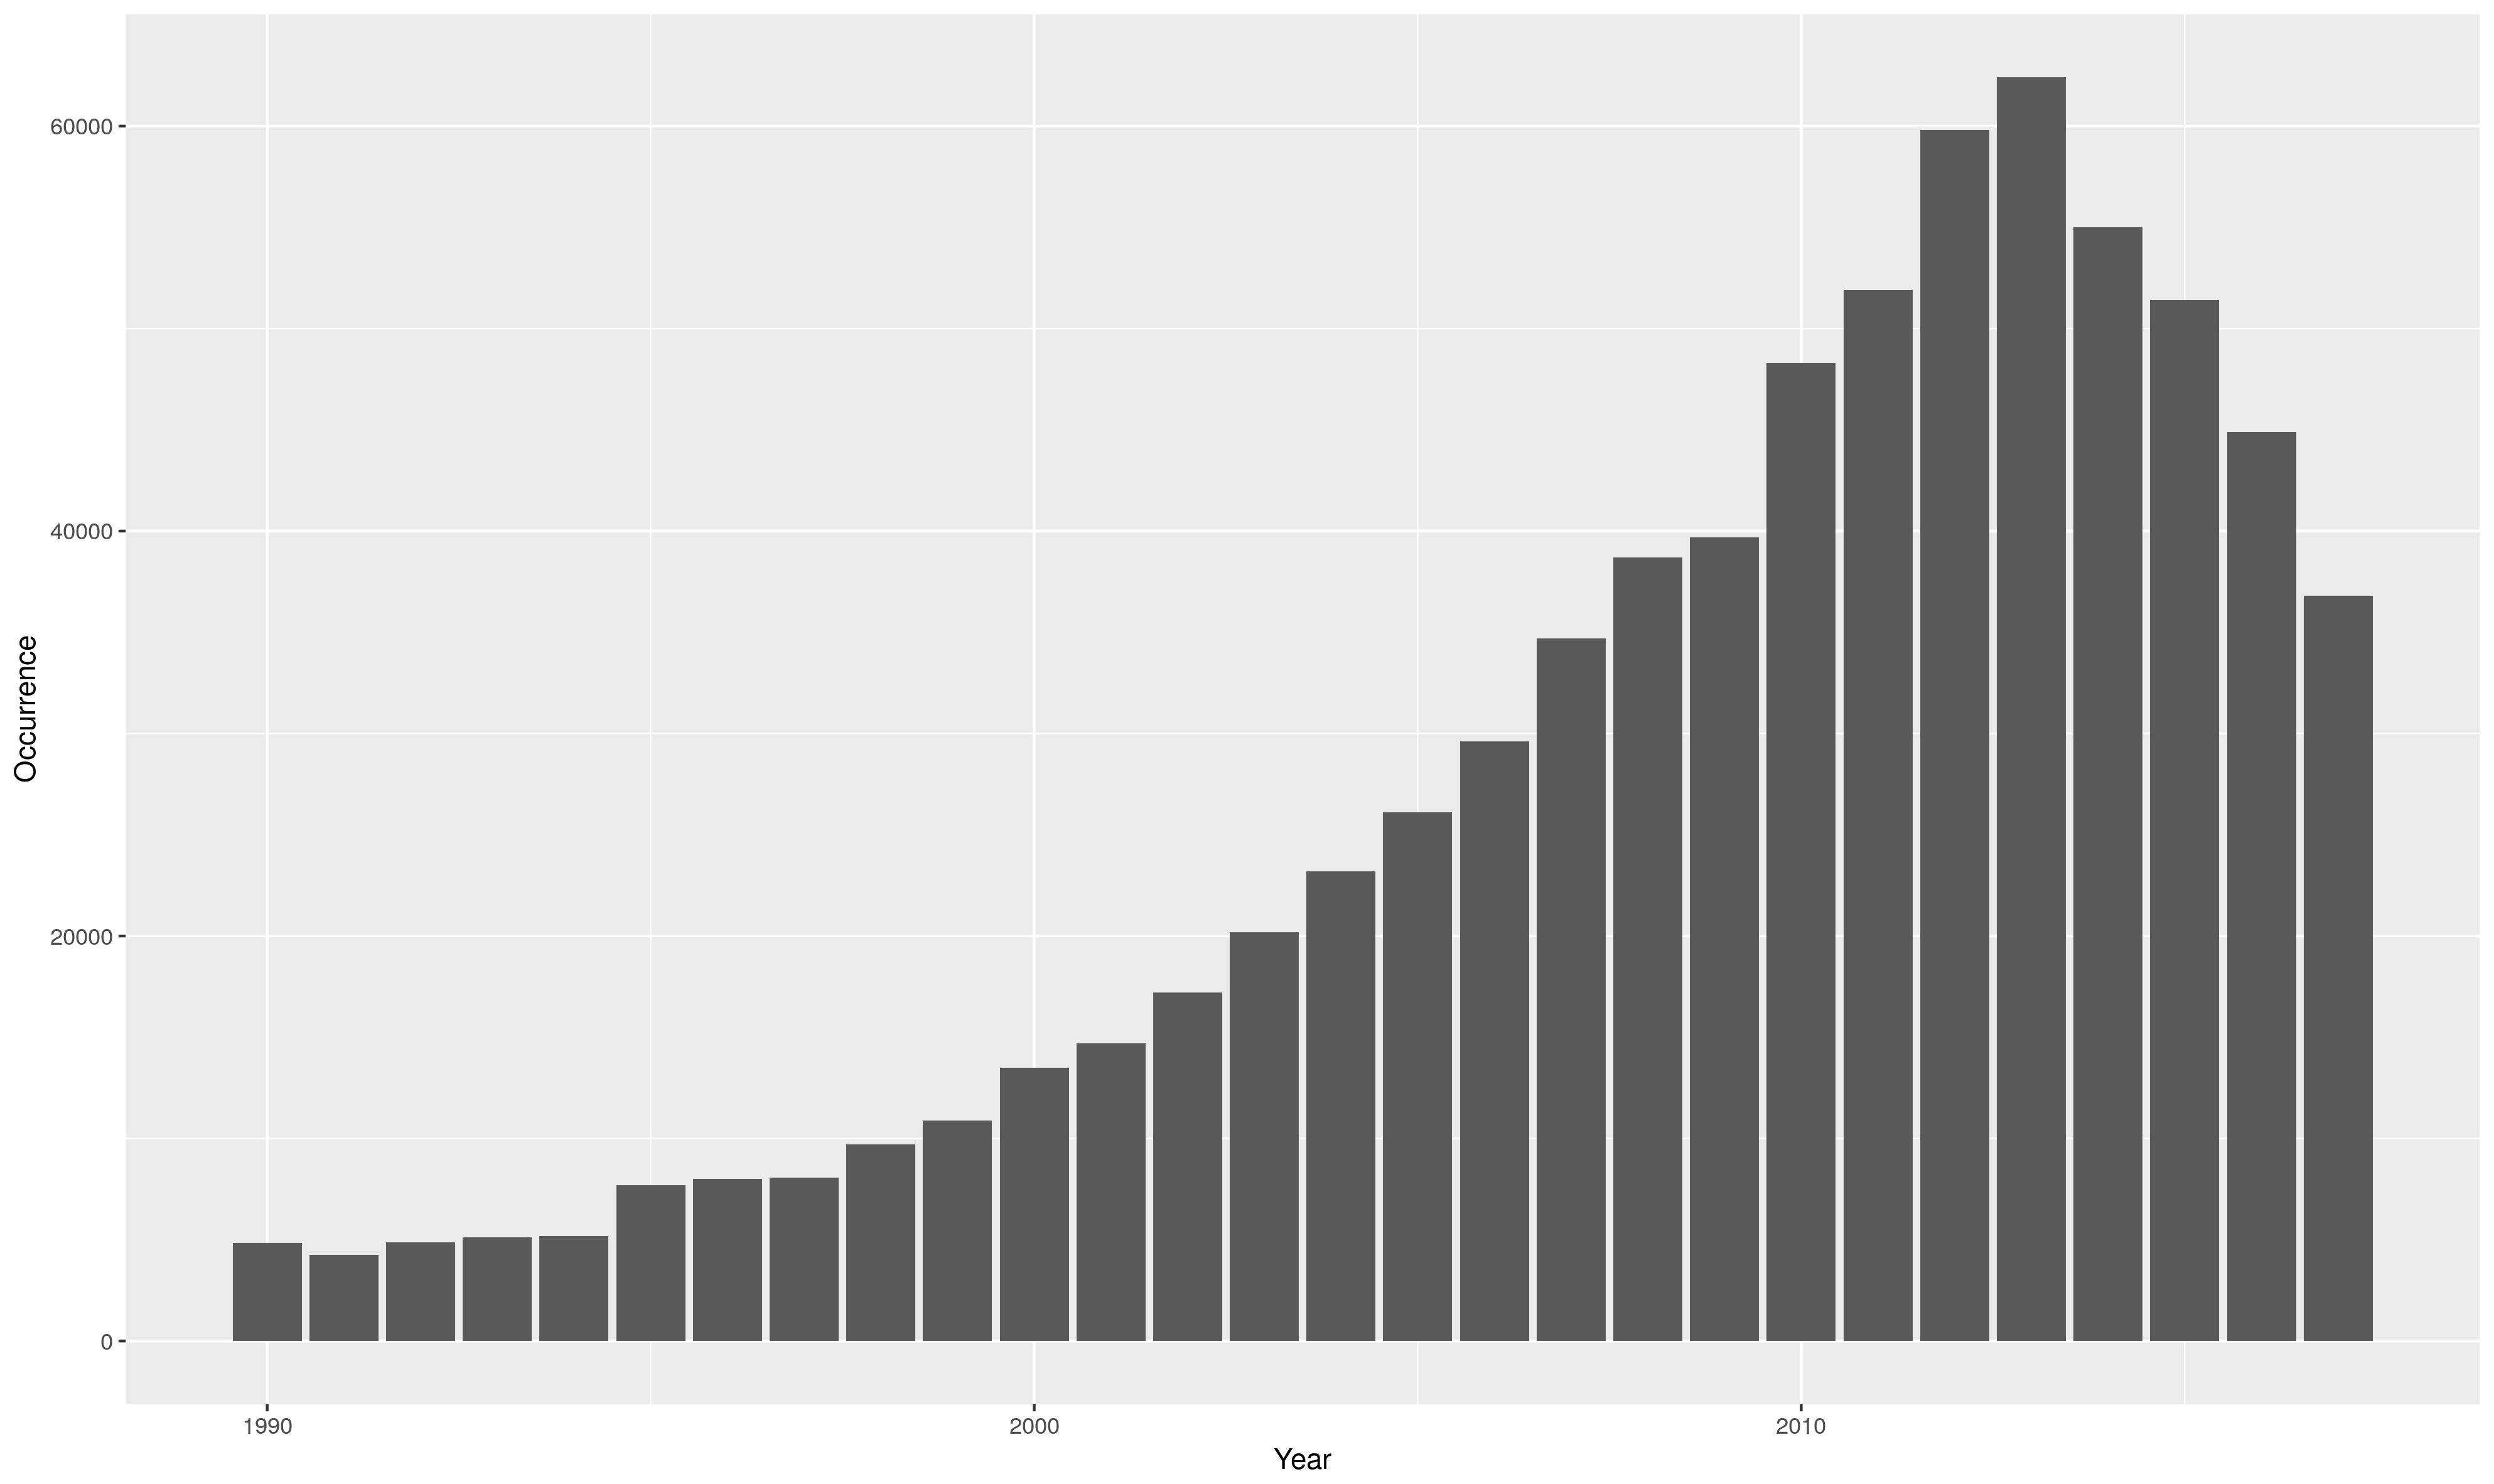
\includegraphics[width=\textwidth]{Images/occurence.png}	
	\label{fig:occurrence}
	\caption{Occurrence of Green Supply Chain in papers indexed by Google Scholar}	
\end{figure}
\\
Although Green Supply Chain management is perceived as a game changer in order to unleash long-term sustainability of a business, it's worth noting the lack of a univocal definition. In fact, some of the academics see GSCM as a process\cite{Gilbert2001}, more specifically a "greening process" from this school of thought belongs the line of thought that the management has the duty of incorporating the environmental criteria along with all the organizational value creation process. Another definition sees the Green Supply Chain as a set of policies whose focus is to raise environmental concern along the production, distribution process\cite{Zsidisin2001}. In this paper is used a two-level definition the first definition is a formal one that builds from the concept of Supply Chain Management as defined by the Council of Supply Chain Management Professionals; the second is a substantial one and deals with the operations affecting the "green" practices inside the firm.
\\
In formal terms, Green Supply Chain may be defined as the series of interconnected activities across the border of different enterprises that adds value to the goods and services from the sourcing to the market. Its aim is to improve performance in measures of sustainability, cost reduction, emission reduction. Whereas Supply Chain Management sets its objectives to maximize profits and minimize waste, in economic terms, Green Supply Chain sets its objectives even further, posing as its ultimate mission to lower the ecological impact that a firm or a series of them has in their day to day operations. 
Such green operations\cite{srivastava_green_2007}\cite{Zhu2008} constitutes the substantial definition of Green Supply Chain Management, these operations are:
  \begin{itemize}
    \item Green Manufacturing and Re-manufacturing: is the process of controlling and reutilizing material in the manufacturing, in order to limit waste creation\cite{urvashi_green_2013};
    \item Green Design: is an approach put in place to promote the environmental quality of a certain product or service,  by reducing negative impacts on the natural environment; an example could be the automatic switch of the television after a period of idleness\cite{ceschin_evolution_2016}; and
    \item Green Operations in general: by green operation is intended any type of activity which does not fall into the two categories mentioned above but is characterized by a "green" attitude as for example the optimization of the offices' consumption through a remote-working policy;
  \end{itemize}
  
  Apart from the definition and its importance in the business field is important to focus the attention of the main drivers affecting this change, in fact such drivers are many and involves the overall ecosystem of the firm (external drivers), and even the firm (internal drivers) in its reactions to this drivers plays a key role in setting its environmental behavior that may be reactive, focused, opportunistic, and proactive\cite{YolLee2007}. Speaking about the external drivers, they fall into four main categories:
  \begin{itemize}
	  \item Legal frameworks: embraces all the set of laws either soft or hard laws, that implies certain standards and regulation over the operations provided along the supply chain;
	  \item Customer relations and concerns: in this category pertain every possible action overtaken by the end-users who can force their pressure on the firm enacting nonbuying campaign and manifestation in general;
	  \item Supplier/distributors relations: the actions pertaining to this category are similar to the ones of the customers, the only difference is that since are enacted    by entities that are constituting the supply chain they can provoke major issue in providing good and services on the market;
	  \item External stakeholders, this category embraces all the stakeholders that do not follow in the categories of either customers and suppliers, which may include stockholder, agents involved by the environmental behavior of the firm, is an example the households living near the production plan, etc...
  \end{itemize}
Since the model proposed it's aimed at setting a Green Supply Chain network of products from the procurement sites to the end user market which is stated to be the Euro Zone; it's necessary to highlight the set of norms that characterize such market and in particular a specific attention will be given to the norms concerning electrical products.

  \subsection{The legal framework: a European perspective}
  In the market under scope which is the European one, there are several legislations concerning the environmental impact of certain e-Products\footnote{for e-Products, is intended an electrical or electronic equipment such as computers, TV-sets, fridges, cell phones and other electronic appliances}. The most important are:
  \begin{itemize}
    \item Waste Electrical \& Electronic Equipment (WEEE);
    \item Restriction on Hazardous Substances (RoHS);and
    \item Ecodesign Requirement for Energy-using Product (EuP).
  \end{itemize}

  Such legal frameworks act at different levels from the sourcing to the customer involving community member States. The following flowchart illustrates this differences.

  \begin{figure}[ht]
    \centering

    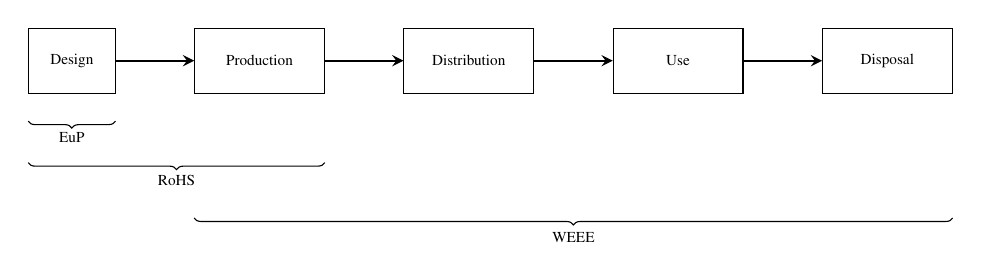
\begin{tikzpicture}[scale=0.8, every node/.style={scale=0.55}]
    \node (start) [startstop] {Design};
    \node (process1) [process, right=of start] {Production};
    \node (process2) [process, right=of process1] {Distribution};
    \node (process3) [process, right=of process2] {Use};
    \node (process4) [process, right=of process3] {Disposal};

    \draw [arrow] (start)--(process1);
    \draw [arrow] (process1)--(process2);
    \draw [arrow] (process2)--(process3);
    \draw [arrow] (process3)--(process4);

    \draw[decorate,decoration={brace,mirror,raise=10pt}]
    (start.south west) -- (start.south east) node[below, midway, yshift = -22]  {EuP};
    \draw[decorate,decoration={brace,mirror,raise=25pt}]
    (start.south west) -- (process1.south east) node[below, midway, yshift = -50]  {RoHS};
    \draw[decorate,decoration={brace,mirror,raise=45pt}]
    (process1.south west) -- (process4.south east) node[below, midway, yshift = -88]  {WEEE};

    \end{tikzpicture}
    \caption{Legislation affection}
  \end{figure}

  In the following subsection, an additional overview is given to such legislations.

\subsubsection{Waste Electrical \& Electronic Equipment}
  The Waste Electrical \& Electronic Equipment also called WEEE is ruled in the European Community by Directive 2002/96/EC now repealed by the Directive 2012/19/EU. The objectives of the policy are, to preserve, protect and improve the quality of the environment, to protect human health and to utilize natural resources prudently and rationally. That policy is based on the precautionary principle meaning that the polluter should pay for its damage. Is important to notice that in the European market such directive is impacting all the community members is not perfectly homogeneous ways because of the implementation which is remitted to the local authorities. This problem may incur in potential elusive behavior as highlighted by the German firms who exploited gaps in the law which have allowed them to move large amounts of WEEE declared for recycling to developing economies including India, China, Nigeria and Eastern Europe \cite{ongondo_how_2011}. Despite such cases, the overall impact of this directive is mostly positive as highlighted by the Eurostat data here exposed.

  The WEEE Directive currently sets a minimum collection target of 4 kg per year per inhabitant for WEEE from households. From 2016, the minimum collection rate shall be 45\% calculated on the basis of the total weight of WEEE collected. Where the WEEE is calculated with the following formula:
  $$
  W (n) = \sum{t = t_0}_{n} POM \cdot L^p(t,n)
  $$
   Where $W(n)$ refers to the specific quantity of electrical and electronic waste for a specific year, $POM(n)$ is the quantity of new electrical component injected in the market and $L$ is the discard-based lifespan profile for the electrical component injected in the market. From the graph proposed below is possible to see how the target of minimum collection of 4 kg per year per inhabitant for WEEE from households was achieved by all the countries in the Eurozone however not all the countries has the same collection rate, meaning that some of them may have introduced legislation that complies only with the minimum target of the directive, leaving the households with the freedom to dispose of their WEEE in an unconventional manner. Clearly, this means for the enterprises fewer obligations on the collection of e-Products, but at the same time fewer products to be recycled and less opportunity of remanufacturing.

  \begin{figure}
  \centering
  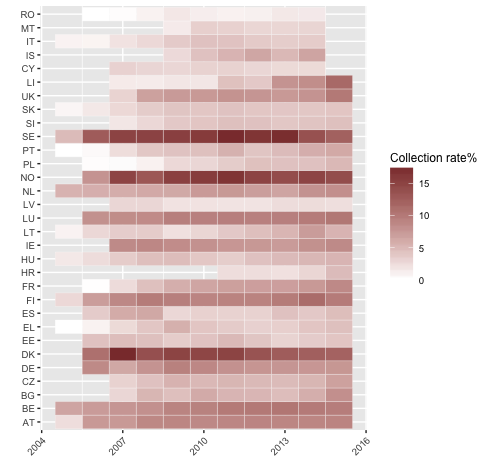
\includegraphics[width=0.8\linewidth]{Images/heatmap.png}
  \caption{Kilograms of WEEE collected per capita}
  \end{figure}

\subsubsection{Restriction on Hazardous Substances}
  The Restriction on Hazardous Substances also called RoHS is represented by the Directive 2017/2102 (RoHS 2 recast). The scope is the restriction on the use of certain hazardous substances in electrical and electronic equipment (EEE) such as lead, mercury, cadmium, hexavalent chromium etc... In such case, as opposed to the WEEE the RoHS directive acts as a barrier to the products containing such minerals and not when they become waste. In considering such regulation is worth noting that there are no differences between the dimension of the distributing entity, meaning that small businesses, as well as large businesses, are equally affected by these restrictions. The only amendment is given to the batteries that may exceed such restriction.

\subsubsection{Ecodesign Requirements for Energy-using Product}
  The Directive 2009/125/EC is meant to deal with Ecodesign regulations. Ecodesign regulations require manufacturers to decrease the energy consumption of their products by establishing minimum energy efficiency standards. In particular, The Ecodesign Directive provides a consistent legal framework for improving the environmental performance of products setting out a minimum mandatory requirement for the energy efficiency of these products. In case of the design of IT networking products such as routers and switches the firms are obliged by such directive to implement some ecodesign features such as the maximum wattage of 1W in case of off mode or a standby maximum consumption of 2W. Such measure per se does not impact in any case the supply chain since they are just additional features that have to be implemented in the products sold in Europe.

\pagebreak 

\section{A state-of-the-art review: mathematical modeling in SCM}
  As proposed by the Council of Supply Chain Management Professionals, the Supply Chain Management (SCM) is the planning and the management of all activities involved in sourcing and procurement, conversion, and logistics as well as coordination and collaboration with the entities. The problem arising from such activities seems to be well addressed by mathematical modeling, other advantages of such approach are the economic sustainability and the possibility to scale the model in order to address different situations.
  From the comprehensive review built by Muna et al. \cite{mula_mathematical_2010} the methods used by the academic world and the specific situations they tried to model, are:
  \begin{itemize}
	  \item Linear Programming: order quantity definition by means of decentralization\cite{jung_order_2008}, production and distribution planning taking into account country specific regulations\cite{Oh_Karimi_2006}, multiple points of sales planning\cite{Kanyalkar_2005};
	  \item Mixed Integer Linear Programming: network optimization and routing configuration\cite{romo_optimizing_2009}, distribution planning in an environment with just a production plant and many distribution centers\cite{Rizk_Martel2008};
    \item Non Linear Programming: optimization of production, transport and inventories\cite{benjamin_analysis_1989};
    \item Multi Objective Programming: replenishment production and distribution planning with conflicting objectives simultaneously\cite{torabi_interactive_2008}, master planning\cite{Chern_Hsieh_2007};
    \item Fuzzy Mathematical Programming: distribution allocation considering different products and production/distribution centers\cite{Liang_Cheng_2009};
    \item Stochastic Programming: addressing demand uncertainty accounting for the probability distribution\cite{Gupta_Maranas_2003};
    \item Heuristics Algorithms and Meta-Heuristics; and
    \item Hybrid Models.
  \end{itemize}

Is worth noting how the majority of the models pertain to the category of Mixed Integer Linear Programming, this may be due to the fact that is probably one of the simplest and most reliable methods that can be used to solve such problems, however, this simplicity comes with some costs such as the focus on a single linear objective function with linear constraints whereas in reality different objectives have to be taken into account as for example the manager preferences toward greener choices. Another interesting topic brought into light by Aouni \cite{azimian_supply_2017} is that such models are generally deterministic, where in reality such assumption does not hold most of the time, for example, the demand forecast can't be deterministic at all and derives from a stochastic process. This lack of deterministic variable lies also in case of the procurement where the price of a commodity is said to follow a sort of stochastic process, and an order may be placed several days after the decision to make it, however this does not apply to business depending on specific materials which are not sold as commodity, as for example processors or motherboards. Both of these situations, namely the fuzziness of the DM and the stochastic process of the demand will be modeled using two variances from the plain vanilla GP, that is Stochastic Goal Programming and Fuzzy Goal Programming.

  \subsection{Stochastic Optimization: a Goal Programming perspective}
 As previously stated, deterministic models seem to be the preferred choice by practitioners and academics whereas in reality there's a certain level of uncertainty that comes into play when deciding over the planning of the supply chain. When a decision maker is facing a multitude of random objectives is stated to face a multi-objective stochastic program (MSP). Because of its flexibility Goal Programming turned to be a very powerful tool in modeling multi-objective deterministic problem. The formulation originally proposed by Charnes and Cooper\cite{charnes_optimal_1955} was built for deterministic scenarios, and with further development, starting from Contini\cite{Contini1968}, a newer branch was developed which accounted for nondeterministic situations, namely stochastic Goal Programming. The resulting model is generalized as follow:
\begin{mini!}
	{\tilde{\delta^+},\tilde{\delta^-}}{\sum_{i=i}^{N}\tilde{\delta^+_i} +\tilde{\delta^-_i}}{}{}
	\addConstraint{f_i(x)-\tilde{\delta^+_i}+\tilde{\delta^+_i}}{=\tilde{g_i},}{\forall i \in N}
	\addConstraint{x\in h_s(x)}{\leq 0}{\forall s \in M}
	\addConstraint{\tilde{\delta^+},\tilde{\delta^-}}{\geq 0}{}
\end{mini!}
Where the goal variable $\tilde{g}$ is said to follow a certain probability distribution. A very common solution to deal with such stochastic problem is transform the undetermined problem into a deterministic one (also called deterministic equivalent formulation). Looking at the general formulation made before, if $\tilde{g}$(or the $\tilde{g_i}$ vector in our case) is said to follow a normal distribution $N(\mu;\sigma^2)$, therefore we can reformulate the program in its equivalent formulation\cite{azimian_supply_2017}
\begin{mini!}
	{\tilde{\delta^+},\tilde{\delta^-}}{\sum_{i=i}^{N}\tilde{\delta^+_i} +\tilde{\delta^-_i}}{}{}
	\addConstraint{f_i(x)-\tilde{\delta^+_i}+\tilde{\delta^+_i}}{=\mu_i,}{\forall i \in N}
	\addConstraint{x\in h_s(x)}{\leq 0}{\forall s \in M}
	\addConstraint{\tilde{\delta^+},\tilde{\delta^-}}{\geq 0}{}
\end{mini!}

  \subsection{Fuzzy Goal Programming}
  Fuzzy GP is a subset of Goal Programming models that uses fuzzy sets, which were firstly developed by Zadeh\cite{Zadeh_1965}. The main advantage of fuzzy sets is that they can better model the level of imprecision of a particular feature of the model, usually, such imprecision deals with the target goal, but this does not mean that fuzzy target goals are the only factors that can be enhanced via fuzzy sets. The fundamental part of a fuzzy GP is the membership function (or in case of multiple fuzzy sets, functions)characterizing the shape of the fuzzy sets, and also how it penalizes values above and below some predetermined thresholds. In fuzzy GP the most common membership functions used are: (1) right-sided, used to penalize positive deviations; (2)left sided, used to penalize negative deviations; (3) triangular shaped, in this case the membership function penalizes both positive and negative deviations;(4) trapezoidal shaped, similar to the triangular shaped, since both positive and negative deviations are penalized, however in this case we allow for an interval of complete satisfaction.
  Recent works of fuzzy GP were made in the field of engineering where fuzzy sets where used to model the perfect selection of wind turbine in order to fully unleash the potential of each particular sites\cite{Rehman2017}; in the field of management, where a case study of wastewater treatment was proposed, combining both fuzzy GP and Stochastic GP\cite{Diaz-Madronero2018}; and in the field of social sciences where fuzzy GP was applied in analyzing environmental and sustainability goals of a country spotting improvement opportunities, requirement of efforts and implementing the sustainable development plans\cite{Nomani2016}.   
  \pagebreak

\section{Model formulation}
The hybrid model developed is based on the supply chain concept developed by Santoso\cite{Santoso_Ahmed_Goetschalckx_Shapiro_2005}plus the integration of supporting activities as enunciated by Porter\cite{CompetitiveAdvantage}in his concept of the value chain. Apart from these features, as the model is built with the concept of Green Supply Chain management seemed necessary to enhance the basic capabilities of an open loop supply chain network with the characteristics of a typical reverse supply chain network (which is intended to be in closed loop fashion). Because of the reverse supply chain network, a series of new entities have been introduced, namely the recollection points, which in our case are the same retail stores, and the recycling point that has to comply both with regulation and with management expectation in terms of recycled products. Therefore, a fuzzy goal is created using the fuzzy goal programming formulation developed by the \cite{YAGHOOBI2008}, such formulation, as reported previously, tries to capture the DM preferences about units recycled and the bottom line imposed by regulations.

\subsection{Open Loop Supply Chain}
In a very general open loop supply chain model the materials after been purchased pass through a series of entities where they are transformed into goods (operation activities), then follows the process of outbound logistics where the goods produced has to reach their specific market for satisfying consumer demand, however, such last operation is subject to certain costs, such as the sales force and marketing campaigns which are, generally, managed and supervised by the national retail stores in each specific country.
A general formulation of such model is given by Santoso and is formulated as follows:
\begin{mini!}
	{y,x}{\sum_{i=1}^{P} c_i y_i  + \sum_{k=1}^{K} \sum_{(i,j)=1,1}^{A} q_{ij}^{k}x_{ij}^{k}}{}{}
	\addConstraint{\sum_{i=1}^{N} x_{ij}^k - \sum_{l=1}^{N} x_{jl}^k}{=0,}{\forall j \in P, \forall k \in K}
	\addConstraint{\sum_{i=1}^{N} x_{ij}^k}{\geq d_{j}^k,}{\forall j \in C, \forall k \in K}
\addConstraint{\sum_{j=1}^{N} x_{ij}^{k}}{\leq s_{i}^{k},}{\forall i \in L, \forall k \in K}
	\addConstraint{\sum_{k=i}^{K} r_{j}^k \cdot \sum_{i=1}^{N}x_{ij}^k}{\leq m_j y_i,}{\forall j \in P}
	\addConstraint{x \in \varmathbb{R}^+}{y \in Y[0,1]}{}
\end{mini!}

Where the objective function $(3a)$ is to minimize both the variable and fixed costs (here represented by the cost of building a plant) of a particular supply chain network.
The constraint posed in $(3b)$ serves to maintain the flow constant in each passage(so-called flow conservation) it serves to balance the net inflow with the net outflow; the second and third constraint here represented by $(3c)$ and $(3d)$ are respectively controlling the volume of the demand (receiver side) and the supply (supplier side) of the supply chain network; whereas the fourth constraint $(3e)$ is used to control the capacity of each node. Lastly, the $x$ variable, indicating the flow of goods has to be positive and the variable $y$ indicating the effective construction of the plant to assume a value that is either 1 or 0, in other terms $y$ is said to be binary. 
\\
However the model is complete from a point of view of supply chain modeling it's worth noting that such model does not implement any support activities, whereas the Porter model mentions them. Therefore the hybrid model will contain a set of constraint indicating such activities and a new objective function embracing this change.

\begin{figure}[ht]
  \centering

  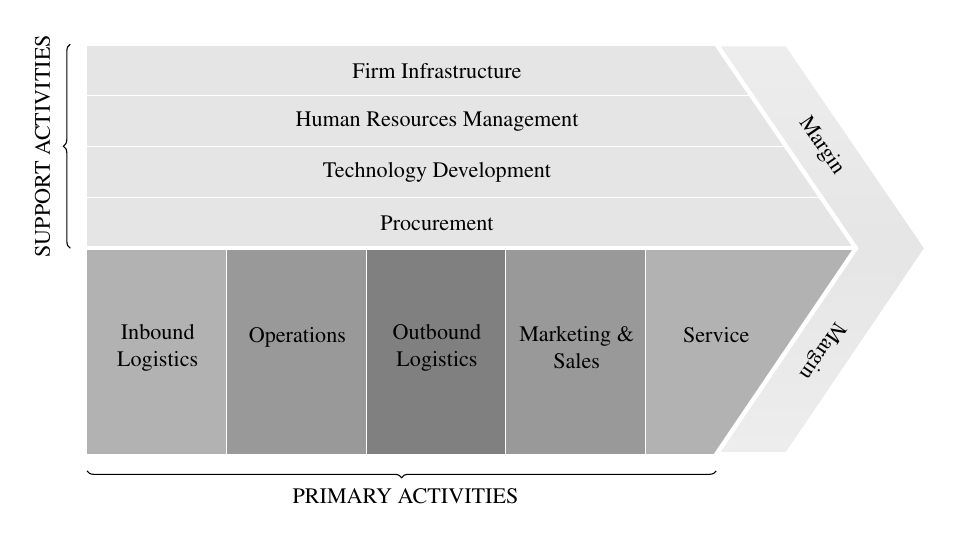
\begin{tikzpicture}[scale=0.8, every node/.style={scale=0.8}]
  \matrix (mat) [table]
  {
  |[fill=colfour]| & |[fill=colfour]| & |[fill=colfour]| & |[fill=colfour]| & |[fill=colfour]| &  \\
  |[fill=colfive]| & |[fill=colfive]| & |[fill=colfive]| & |[fill=colfive]| & |[fill=colfive]| &  \\
  |[fill=colsix]| & |[fill=colsix]| & |[fill=colsix]| & |[fill=colsix]| & |[fill=colsix]| & |[fill=colsix]| \\
  |[fill=colseven]| & |[fill=colseven]| & |[fill=colseven]| & |[fill=colseven]| & |[fill=colseven]| & |[fill=colseven]| \\
  |[fill=colone]| & |[fill=coltwo]| & |[fill=colthree]| & |[fill=coltwo]| & |[fill=colone]| & |[fill=colone]|  \\
  |[fill=colone]| & |[fill=coltwo]| & |[fill=colthree]| & |[fill=coltwo]| & |[fill=colone]| & |[fill=colone]|  \\
  |[fill=colone]| & |[fill=coltwo]| & |[fill=colthree]| & |[fill=coltwo]| & |[fill=colone]| & \\
  |[fill=colone]| & |[fill=coltwo]| & |[fill=colthree]| & |[fill=coltwo]| & |[fill=colone]| &  \\
  };

  \foreach \row in {2,3,4}
  \draw[white] (mat-\row-1.north west) -- (mat-\row-6.north east);
  \draw[white,ultra thick] (mat-1-1.north west) -- (mat-1-6.north east);
  \draw[white,ultra thick] (mat-5-1.north west) -- (mat-5-6.north east);

  \foreach \col in {2,3,4,5}
  \draw[white] (mat-5-\col.north west) -- (mat-8-\col.south west);

  \node[fill=colfour] at (mat-1-3) {Firm Infrastructure};
  \node[fill=colfive] at (mat-2-3) {Human Resources Management};
  \node[fill=colsix] at (mat-3-3) {Technology Development};
  \node[fill=colseven] at (mat-4-3) {Procurement};
  \node at ([yshift=-10pt]mat-6-1) {\parbox[t]{2cm}{\centering Inbound Logistics}};
  \node at ([yshift=-10pt]mat-6-2) {\parbox[t]{2cm}{\centering Operations \\\mbox{}}};
  \node at ([yshift=-10pt]mat-6-3) {\parbox[t]{2cm}{\centering Outbound Logistics}};
  \node at ([yshift=-10pt]mat-6-4) {\parbox[t]{2cm}{\centering Marketing \& Sales}};
  \node at ([yshift=-10pt]mat-6-5) {\parbox[t]{2cm}{\centering Service \\\mbox{}}};
  \node[rotate = 90] at ([xshift=-52pt]mat-3-1.north) {SUPPORT ACTIVITIES};
  \node at ([yshift=-19pt,xshift=-0.5cm]mat-8-3.south) {PRIMARY ACTIVITIES};

  \fill[white] (mat-1-5.north east) -- (mat-5-6.north east) -- (mat-1-6.north east) -- cycle;
  \fill[white] (mat-8-5.north east) -- (mat-5-6.north east) -- (mat-8-6.north east) -- cycle;

  \shade[top color=colfour!70,bottom color=colfour!70,middle color=colseven,draw=white,ultra thick]
  (mat-1-5.north) -- (mat-5-6.north) -- (mat-8-5.south) --
  (mat-8-5.south east) -- (mat-5-6.north east) -- (mat-8-5.south east) --
  (mat-5-6.north east) -- (mat-1-5.north east) -- cycle;

  \begin{scope}[decoration={markings,mark=at position .5 with \node[transform shape] {Margin};}]
  \path[postaction={decorate}]
  ( $ (mat-1-5.north)!0.5!(mat-1-5.north east) $ ) -- ( $ (mat-5-6.north)!0.5!(mat-5-6.north east) $ );
  \path[postaction={decorate}]
  ( $ (mat-5-6.north)!0.5!(mat-5-6.north east) $ ) -- ( $ (mat-8-5.south)!0.5!(mat-8-5.south east) $ );
  \end{scope}

  \draw[decorate,decoration={brace,mirror,raise=6pt}]
  (mat-1-1.north west) -- (mat-5-1.north west);
  \draw[decorate,decoration={brace,mirror,raise=6pt}]
  (mat-8-1.south west) -- (mat-8-5.south);
  \end{tikzpicture}

  \caption{Porter's Value Chain}
\end{figure}

Such activities are a fundamental part of the supply chain that serves as glue with the supply chain steps to the deliver the value to the end-customer. Therefore the hybrid model should take them into account, a revised version then is proposed.

\begin{mini!}
  {x}{\sum_{k=1}^{K} \sum_{(i,j)=1,1}^{A} q_{ij}^{k}x_{ij}^{k} + \sum_{i=1}^{N} c_i \sum_{k=1}^{K} \sum_{(i,j)=1,1}^{A}x_{ij}^{k}}{}{}
  \addConstraint{\sum_{i=1}^{N} x_{ij}^k - \sum_{l=1}^{N} x_{jl}^k }{=0,}{\forall j \in P, \forall \in K}
  \addConstraint{\sum_{i=1}^{N} x_{ij}^k}{\geq d_{j}^k,}{\forall j \in C, \forall k \in K}
\addConstraint{\sum_{j=1}^{N} x_{ij}^{k}}{\leq s_{i}^{k},}{\forall i \in L, \forall k \in K}
\addConstraint{\sum_{k=i}^{K} r_{j}^k \cdot \sum_{i=1}^{N}x_{ij}^k }{\leq m_j,}{\forall j \in P}
\addConstraint{\sum_{i=1}^{N} q_{i}^j}{= n_j,}{\forall j \in P}
\addConstraint{x \in \varmathbb{R}^+ }{,}{}
\end{mini!}

In formulating our hybrid model is not taken into account the fixed cost of building a plant, this happened for two reasons. The first reason is the consideration of the cost of building a plant as a sunk cost and therefore it should not influence the economic decision on whether to allocate a particular quantity of goods on a specific plant. Secondly, since we use the Activity Based Cost method, the focus will be on the activities that contribute to creating the marginal cost of the good in the supply chain.

\subsection{Closed Loop Supply Chain}
In the previous sections a model of an open loop supply chain was presented, however in green supply chain something as an open loop supply chain network does not exist, this is because of the after-life treatment of the products sold by the company. Such procedure is also enforced by hard laws (as analyzed in the specific section). Therefore the revised model will have to capture these features. The closed loop supply chain network will be enunciated as follow:

\begin{mini!}
	{x}{\sum_{i=1}^{I}\sum_{j=1}^{J}\sum_{k=1}^{K} c^f_{ijk} x^f_{ijk}  + \sum_{k=1}^{K}\sum_{l=1}^{L}\sum_{i=1}^{I0} c^r_{kli} x^r_{kli}}{}{}
\addConstraint{\sum_{i=1}^{I}\sum_{j=1}^{J} x^f_{ijk}}{= d_k,}{\forall k \in K}
\addConstraint{\sum_{l=1}^{L}(\sum_{i=0}^{I} x^r_{kli} - x^r_{kli})}{= w_k,}{\forall k \in K}
\addConstraint{\lambda \sum_{i=1}^{I0} x^r_{kli}}{\leq x^r_{il},}{\forall k \in K ,\forall l \in L}
\addConstraint{\sum_{k=1}^{K} \sum_{i=1}^{L} r_k x^r_{kli}}{\leq \sum_{k=1}^{K} d_k,}{\forall i \in I}
\addConstraint{x \in \varmathbb{R}^+ }{,}{}
\end{mini!}

The model enunciated minimizes two different flow costs, namely the one implying the forward flow, the one from the production plant to the consumer and the reverse flow that follows the opposite direction, namely from the consumer to the production plant passing through ad-hoc dismantling plants. The constraints applied to such models are therefore a combination of both forward flow constraints, mitigated from the classical open loop supply chain, and the reverse flow constraints. The constraint at $5b$ is stating that the forward flow must equal the demand of the customer at a particular retailing site; where instead the constraint at $5c$ is enunciating the amount of waste that will not be part of the recycling process. The constraint at $5d$ focuses on imposing a threshold in which the units recycled will not be of any advantage for the production plan and therefore will constitute an additional waste. Lastly, constraint $5e$ that states the inequality about the products collected that should not exceed the products delivered at a $k$ general retail store. 
\\
\\
The model presented, however, does not implement any decision maker preferences toward recycling level goals ($\lambda$ is only a crisp value that affects the plant necessity) nor any legal boundaries on which the recycling center has to be submitted. Because the electronic waste turns out to be a resource for the firm is necessary to model the fuzziness of such desire expressed by the DM, and therefore the implementation of a Fuzzy set\cite{Zadeh_1965}, turns out to be the best choice; such set has a membership function defined as:
$$
\mu [f_k(x)]=
\begin{cases}
1 & f_k(x) \geq b_k \\
1-\frac{b_k-f_k(x)}{n_{max}} & b_k -n{max} \leq f_k(x) \leq b_k \\
0 & f_k(x) \leq b_k - n_{max}
\end{cases}
$$

The defined set penalizes the negative occurrences from the target demanded by the decision maker, and at the same time guarantees a bottom line coherent with the local legislation. The following figure represents the graphical interpretation of the fuzzy set for a generic dismantling plant, whereas the $n_{max}$ represent the legal boundaries in which any lower achievement will not be tolerated, conversely $b_k$ is the goal sought by the decision maker as optimal, this may be due to some particular public image concerns enacted by the DM. 

\subsection{The Goal Programming model}
Since we are facing a multitude of goals; some of them aims at the minimization of the transportation costs of both the forward flow and the recycling flow; some are set in order to control the supporting activities, and ultimately some are trying to capture the preference and necessities of the DM.
Because of this multitude of goals a multi-criteria decision analysis tool was used, namely the Goal Programming approach. In this approach, the goal is to minimize a set of deviational variable applied to our desired goals.
The model proposed builds from the concept of open loop supply chain (it's possible to see it in the first soft constraints) taking into account even the support activity costs of each individual step in the value chain. Then the supply chain loop is closed implementing the controls on the recycling flow. Additionally, the last soft constraints are an adaptation of the fuzzy set in order to be solved trough linear programming solvers.
\\
\\
The model proposed builds from the concept of open loop supply chain (it's possible to see it in the first soft constraints) taking into account even the support activity costs of each individual step in the value chain. Then the supply chain loop is closed implementing the controls on the recycling flow. Additionally, the last soft constraints are an adaptation of the fuzzy set in order to be solved by linear programming solvers.
\\
\\
In the following sections a deep overview of the objectives, constraints and the model itself will be given.

\subsubsection{Objective function}
The objective function is a function containing all the deviational variables to be minimized as well as their relative weight, in the case under scope the interest is to minimize a series of costs, namely the cost of transportation of the goods from the production plan $ $ to the consumer $K$, and back from the consumer $k$ to the plant $I$ in the latter passage the waste, in other words, the nation collected products will be free of costs since won't be subject to any transportation. Another goal to be minimized is the cost of the supporting activities, this activities lies within each step of the value chain and are not part of any transportation cost, instead they are the cost that sustains the value of the product, a typical support activity cost may be the cost of a marketing campaign in a specific retail store $K$; such costs have to be minimized as well and for a matter of order the deviational variable and their relative weights will follow each particular step of the value chain. Apart from costs, additional goals may be more subtle; this is the case of demand fulfillment. Another goal not implying any cost is the reduction of the product wasted (meaning not recycled).

\subsubsection{Soft Constraints}
The soft constraints are the ones that do not constitute any particular boundary but carries the deviational variables and the goals that are tried to be achieved by the decision maker. The first soft constraints are the ones that deal with the transportation cost of the goods produced; the first flow of transportation is the forward flow and its soft constraint is represented as follows:
$$
\sum_{i=1}^{I}\sum_{j=1}^{J}\sum_{k=1}^{K} c^f_{ijk} x^f_{ijk} - \delta^+_{ijk}=0}
$$
In this case, the goal is to minimize the cost of transportation of the good produced till it reaches the customer, the step that the product has to do in order to reach the customer are two, from the production plant to the distribution center and then to the retail center (indicated with $k$). The same goal has to be achieved by the recycling flow of products returned by the consumer, the soft constraint is similar to the first one and is represented as follows:
$$
\sum_{k=1}^{K}\sum_{q=1}^{Q0}\sum_{i=1}^{I} c^r_{kqi} x^r_{kqi}, - \delta^+_{kqi}=0
$$
The peculiarity of this passage is given by the set $Q0$ which is not only the set of possible dismantling plant (the flow now is from consumer $K$ to dismantling plant $Q0$ till the production plan$I$), but it also includes the set non-collection entity that contains all the units not collected because not necessary to the recycling process.
The other set of soft constraint is given by the support activities and its formulated in the following general form:
 $$
(o^t_s \cdot x^t_s) - \delta^+_s}{=0,}{\forall s \in S}
 $$
 Where the $t$ stands for the type of flow that can be forward $f$ or recycling $r$ whreas the index $s$ represent each specific step on the value chain that can be $i$ for a production plant, $j$ for the distribution center, $k$ for the retailing center and $q$ for dismantling plant.
 COnstitutes a soft constraint also the achievement of the demand by the supplied product, the deriving constraint is reported as follows:
 $$
x_k + \tilde{\delta^-_k} = EV[d_{k}],\forall k \in K
 $$
 In this case, the demand is not a fully determined value but is determined through a stochastic process that; in this case, the deterministic equivalent formulation is used by calculating the expected value of the demand of each retailing center.
 Changing the perspective from the forward flow to the recycling flow some additional soft constraints are necessary; these constraints are respectively the fuzzy preferences of the DM and the minimization of the waste produced. The first soft constraint is given by the following equations:
 $$
 x_q + \delta^-_q = b_{k},\forall q \in Q0
 $$
 $$
 \mu_q + \frac{\delta^-_q}{n_{max}}= b_{k},\forall q \in Q0
 $$
 Where the $n_max$ represent the legal boundary of each dismantling facility, in case the legal boundary is not respected the flow will not be allocated to the facility but to any other disposable facility. Above the lower limit imposed by the legal constraints, we have the goal of the DM that may require a specific target to be achieved by the dismantling plant. The value $\mu_q$ serves to indicate the achievement of this goal, where 0 stands for not achieved at all and 1 indicates full achievement.
 Lastly, we have the goal of cutting waste, which is defined as the amount capable to be collected but not initiated to the recycling process, the specific deviational variable is part of the balance equation of the last node of the supply chain network and is expressed as follows:
$$
\sum_{k=1}^{K} (x^r_{k} - x^r_{i}) - \delta^+_i= w_i,\forall i \in I
$$

\subsubsection{Hard Constraints}
The hard constraints represent the boundaries in which the solution will not be feasible such constraints may be implied by the approach itself, such as the positivity of the deviational variables, or implied by the model, is an example the limit recycled goods that should not be greater then the goods demanded. In the case under scope the hard constraints are:
\begin{itemize}
\item The conservation of the flow: such constraint is needed in the nodes where is not necessary the use of any deviational variable, is an example the flow of goods from the production plant to the distribution warehouse, in that case, there's a need to maintain the balance of the inflow and the outflow to be 0;
\item The upper limit on the recycled product, which cannot be greater than the delivered product;
\item The limit on the product to be recycled to an amount sustainable for the production plant, since the return rate is different from each and every retail, is not worth to collect and recycle all the possible product available but just the quantity necessary for the production plant.
\item The limit on the capacity of each shipment: not every quantity can be shipped from a node to another, this may due to some limitation imposed by the carrier service.
\end{itemize}
From this constraint which is given by the modeled scenario it's necessary to apply other constraints such as the aforementioned positivity of the deviational variables and the value range of the fuzziness membership function value that as to be a number between 0 and 1, this constraint is imposed by the fuzzy set definition.

\subsubsection{Model formulation}
Given the objective function, the soft constraints and the hard ones, the model is proposed in its mathematical form at the end of the following section. In the next section the model will be subject to a weight sensitivity analysis and then the weights will be assigned using an Analytical Hierarchy Process, subsequently the model will be solved via a linear programming solver and the results, with the weights derived from the AHP will be further analyzed.

\begin{mini!}
	{\delta^-,\delta^+}{w^\star_1(\sum_{i=1}^{I} \sum_{j=1}^{J} \sum_{k=1}^{K} \sum_{q=1}^{Q0} \sum_{i=1}^{I} \delta^+_{ijkqi}) + }{}{}
\breakObjective{w^\star_2(\sum_{i=1}^{I} \delta^+_{i} + \sum_{j=1}^{J} \delta^+_{j} + \sum_{k=1}^{K} \delta^+_{k} + \sum_{q=1}^{Q0} \delta^+_{q} + \sum_{i=1}^{I} \delta^+_{i}) + }
\breakObjective{w^\star_3(\sum_{k=1}^{K} \tilde{\delta^-_k}) + }
\breakObjective{w^\star_4(\sum_{q=1}^{Q0} \delta^-_q) + }
\breakObjective{w^\star_5(\sum_{i=1}^{I} \delta^+_i) + }
\addConstraint{\sum_{i=1}^{I}\sum_{j=1}^{J}\sum_{k=1}^{K} c^f_{ijk} x^f_{ijk} - \delta^+_{ijk}}{=0}{}
\addConstraint{\sum_{k=1}^{K}\sum_{q=1}^{Q0}\sum_{i=1}^{I} c^r_{kqi} x^r_{kqi}, - \delta^+_{kqi}}{=0}{}
\addConstraint{(o^f_i \cdot x^f_i) - \delta^+_i}{=0,}{\forall i \in I}
\addConstraint{(o_j \cdot x^f_j) - \delta^+_j}{=0,}{\forall j \in J}
\addConstraint{(o_k \cdot x^f_k) - \delta^+_k}{=0,}{\forall k \in K}
\addConstraint{(o_q \cdot x^r_q) - \delta^+_q}{=0,}{\forall q \in Q0}
\addConstraint{(o^r_i \cdot x^r_i) - \delta^+_i}{=0,}{\forall i \in I}
\addConstraint{x_k + \tilde{\delta^-_k}}{= EV[d_{k}],}{\forall k \in K}
\addConstraint{x_q + \delta^-_q}{= b_{k},}{\forall q \in Q0}
\addConstraint{\mu_q + \frac{\delta^-_q}{n_{max}}}{= 1,}{\forall q \in Q0}
\addConstraint{\sum_{k=1}^{K} (x^r_{k} - x^r_{i}) - \delta^+_i}{= w_i,}{\forall i \in I}
\addConstraint{\sum_{i=1}^{I} x_{i}^f - \sum_{j=1}^{J} x_{j}^f =0 }{,\sum_{k=1}^{K} x_{k}^r - \sum_{q=1}^{Q0} x_{q}^r=0,}{\sum_{q=1}^{Q0} x_{q}^r - \sum_{i=1}^{I} x_{i}^r}
\addConstraint{\lambda \sum_{i=1}^{I} x^r_{kqi}}{\leq x^r_{iq},}{\forall k \in K ,\forall q \in Q0}
\addConstraint{\sum_{k=1}^{K} \sum_{j=1}^{J} r_k x^f_{kji}}{\leq \sum_{k=1}^{K} d_k,}{\forall i \in I}
\addConstraint{r_k x^f_{k}}{=x^r_{k}}{\forall k \in K}
\addConstraint{x \in \varmathbb{R}^+, \mu \in [1,0] }{,}{}
\end{mini!}

\section{Results and Conclusion}
The model was tested with a set of data with the folowing features:
\begin{itemize}
	\item N. 1 production plant;
	\item N. 4 links from production plant to distribution center (NtoN);
	\item N. 4 distribution center;
	\item N. 36 links from distribution center to retail center, in this case the relation were not made nton since each distribution center was allowed to refurnish only some specific retail center and not the entire number of them;
	\item N. 27 retailing centers;
	\item N. 108 links from the retailing center to the dismantiling plants and to the "non collection" plant (NtoN);
	\item N. 4 dismantling plants, including the non collection plant;
	\item N. 4 links from the simantling plan to the production plant (NtoN).
\end{itemize}
The model was solved using the NEOS servers using their API with the data sent through a script built in R, using the R library rneos; since the problem was linear the solver chosen was the CPLEX.

\subsection{Sensitivity analysis}
In the sensitivity analysis, the value of the weights was preemptively determined and the different achievements are reported in the table at the end of the section. The only constraint given was the unit of the sum of the weights, meaning that each weight should be a ratio indicating the importance of the particular objective where 1 is absolute importance (conversely none of the other objectives is important) and 0 is not important at all.

\subsection{Analytical Hierarchical Process for weight determination}

\begin{itemize}
	\item
	\item
\end{itemize}


\newpage 

\printbibliography

\end{document}
